\documentclass[a4paper, 12pt]{report}
\usepackage{setspace}
%\usepackage{subfigure}

\pagestyle{plain}
\usepackage{amssymb,graphicx,color}
\usepackage{algorithm}
\usepackage{algpseudocode}
\usepackage{amsfonts}
\usepackage{latexsym}
\usepackage{amsmath}
\usepackage{pdfpages}
\usepackage[a4paper, margin = 3cm, bottom = 2.5cm]{geometry}
\usepackage[hidelinks]{hyperref}
\usepackage{listings}
\usepackage{xcolor}

\definecolor{codegreen}{rgb}{0,0.6,0}
\definecolor{codegray}{rgb}{0.5,0.5,0.5}
\definecolor{codepurple}{rgb}{0.58,0,0.82}
\definecolor{backcolour}{rgb}{0.95,0.95,0.92}

\lstdefinestyle{mystyle}{
    backgroundcolor=\color{backcolour},   
    commentstyle=\color{codegreen},
    keywordstyle=\color{magenta},
    numberstyle=\tiny\color{codegray},
    stringstyle=\color{codepurple},
    basicstyle=\ttfamily\footnotesize,
    breakatwhitespace=false,         
    breaklines=true,                 
    captionpos=b,                    
    keepspaces=true,                 
    numbers=left,                    
    numbersep=5pt,                  
    showspaces=false,                
    showstringspaces=false,
    showtabs=false,                  
    tabsize=2
}

\lstset{style=mystyle}

\usepackage[
backend=biber,
style=alphabetic,
sorting=ynt
]{biblatex}

\addbibresource{bibliography.bib}

\newtheorem{theorem}{THEOREM}
\newtheorem{lemma}[theorem]{LEMMA}
\newtheorem{corollary}[theorem]{COROLLARY}
\newtheorem{proposition}[theorem]{PROPOSITION}
\newtheorem{remark}[theorem]{REMARK}
\newtheorem{definition}[theorem]{DEFINITION}
\newtheorem{fact}[theorem]{FACT}

\newtheorem{problem}[theorem]{PROBLEM}
\newtheorem{exercise}[theorem]{EXERCISE}
\def \set#1{\{#1\} }

\newenvironment{proof}{
PROOF:
\begin{quotation}}{
$\Box$ \end{quotation}}



\newcommand{\nats}{\mbox{\( \mathbb N \)}}
\newcommand{\rat}{\mbox{\(\mathbb Q\)}}
\newcommand{\rats}{\mbox{\(\mathbb Q\)}}
\newcommand{\reals}{\mbox{\(\mathbb R\)}}
\newcommand{\ints}{\mbox{\(\mathbb Z\)}}

%%%%%%%%%%%%%%%%%%%%%%%%%%


\title{{\vspace{-14em} 
\includegraphics[scale=0.4]{ucl_logo.png}}\\
{{\Huge Generating Novel Motions Based on a Single Training Example}}\\
}
\date{Submission date: 20 April 2024}
\author{DXZB7\thanks{
{\bf Disclaimer:}
This report is submitted as part requirement for the BSc Degree in Computer Science at UCL. It is substantially the result of my own work except where explicitly indicated in the text.The report may be freely copied and distributed provided the source is explicitly acknowledged.}
\\ \\
BSc Computer Science\\ \\
Dr. Yuzuko Nakamura}


\usepackage[parfill]{parskip}
\begin{document}

\onehalfspacing
\maketitle
\begin{abstract}
	This research addresses the challenge of motion generation in computer graphics, traditionally reliant on costly motion capture systems and extensive datasets predominantly featuring human subjects. A novel approach is proposed, utilizing a diffusion model capable of generating diverse, variable-length motions from a single training example. This model is particularly advantageous for generating motions for arbitrary skeleton structures, including animals and imaginary creatures, which significantly deviates from traditional methods that require large, specific datasets. By leveraging the principles of noising and denoising inherent to diffusion processes, the model, employing a CovNext-based architecture and time-step embedding layers, effectively learns to reproduce and diversify motions from minimal input. This approach not only accelerates the training and generation processes but also enhances adaptability to various applications in animation and video games, reducing dependency on manual rigging. The performance of the model is rigorously evaluated through innovative metrics such as reproduction and diversity scores, demonstrating its efficacy in generating coherent and varied motions. This study contributes to the ongoing shift from generative adversarial networks to diffusion models, highlighting their potential in motion generation with limited data input..
\end{abstract}
\tableofcontents
\setcounter{page}{1}


\chapter{Introduction}
Motion generation is a long-standing problem in computer graphics, with several applications in video games, film-making and robotics.
The most common way of acquiring new motion data involves expensive motion capture systems, which require trained experts to operate rigs and perform post-processing on the collected data. Recent advances in the field have focused on neural network based approaches to rectify these issues but come with problems of their own. They often require massive amounts of data to train on and are limited to motions of humans since they are the main subject of motion capture datasets.

This project aims to address these issues by creating a model that can generate diverse motions of a variable length given a single training example. The use of a single training example means that the model loses out on the sheer variety offered by more data-driven models, but offers advantages when it comes to training speed, generation speed and adaptability to arbitrary skeleton structures. For example, the model can be fed a single motion with an arbitrary skeletal structure, such as an animal or imaginary creature, and learn to generate new motions with the same skeletal topology. 

This approach could have several applications in the computer animation domain. For example, an animator could create a single animation for a complicated skeleton, which would then be fed into the proposed diffusion model to generate novel motions. These motions could be used for tasks like crowd animation, where multiple identical skeletons would be able display distinct motions even though they were only trained on a single input motion.

The concept of learning from a single training example has been previously explored in domains such as image generation and motion generation using generative adversarial networks \cite{li_ganimator_2022}. Recently however, they have been shown to perform worse compared to newer diffusion-based models in regards to generative tasks. Diffusion models work by sequentially noising the input data according to some fixed schedule and then using a neural network to denoise from pure noise to generate a result \cite{ho_denoising_2020}. These models are already replacing GANs in image generation tasks, evident by rise of projects like DALL-E \cite{ramesh_zero-shot_2021}, and their suitability for motion generation has been explored in the last couple of years. However, these projects still rely on large datasets and are limited to human motions. Thus, the novelty of my project lies in investigating whether diffusion models are suitable for single-input based motion generation, a task previously dominated by generative adversarial networks (GANs).

\chapter{Related work}

\section{Early Work on Motion Synthesis}
\subsection{Motion texture: a two-level statistical model for character motion synthesis}
This paper \cite{li_motion_2002} introduces a method for creating complex human-figure motions by using "motion textons." Each one is represented by a Linear Dynamic System (LDS) that models the local dynamics of motion segments. The global dynamics, which describe how these segments change and flow into each other throughout a sequence, are handled by a transition matrix. This matrix outlines the likelihood of moving from one texton to another, allowing for both the repetition and variability seen in complex motions.

The method generates new motion sequences by first learning these textons and their distributions from original data. It then uses this information to create new motions that statistically resemble the originals. The authors use a maximum likelihood algorithm to identify and understand the motion textons and their relationships within captured dance motions. 

This approach is used for motion synthesis, where new animations can be automatically created or existing ones can be interactively modified to make new dance routines. This involves defining motion textons with LDS and using a transition matrix to choreograph new sequences from what has been learned.

\subsection{Motion graphs}
This paper \cite{kovar_motion_2002} introduces a new way to create realistic and controllable motion using a collection of motion capture data. The main contribution of this study is the creation of a directed graph, called a "motion graph," which connects different pieces of motion capture clips. This graph combines original motion data and automatically generated transitions, allowing for the creation of new motion sequences by following paths through the graph.

Building a motion graph involves cutting motion capture data into clips and then finding possible points where these clips can be smoothly joined. This process includes checking for transitions by comparing the similarity of motion poses, creating seamless connections using linear blending techniques, and trimming the graph to avoid any dead ends. The selection of transition points pays special attention to the dynamic qualities of human movement, ensuring that the transitions are smooth and maintain the realism of the original data.

A crucial feature of the motion graph technique is its ability to represent a broad range of movements and transitions within a single framework. By showing transitions as edges in the graph, this method provides a structured way to explore the motion database, creating continuous motion sequences that can be adjusted and controlled based on broad user instructions.

\section{Deep Learning Methods}
Recent developments in motion synthesis have moved away from old methods that rely heavily on large datasets. Instead, modern techniques focus on learning from smaller data sources like a single image, motion sequence, or video. This change helps overcome the challenge of producing realistic and varied animations without needing vast amounts of motion capture data. This is especially useful in areas where collecting large-scale data is difficult or impractical such as for arbitrary skeletons.

\subsection{GANimator: neural motion synthesis from a single sequence}
This paper \cite{li_ganimator_2022} uses several layers of GANs to build motion from random noise. These layers are structured to handle different frame rates, giving precise control over the motion's appearance at various levels of detail. Unlike traditional methods that need large sets of motion data, the model only requires one motion sequence to learn.

The GANs include both generators and discriminators, which are trained in stages to capture motion from coarse to fine details. Starting with random noise, the first level generator produces a basic motion sequence. Following generators improve this motion by adding upscaled data from the earlier stage and new noise, leading to a more detailed motion sequence.

In the model, motion is encoded through the movement of the root joint and the rotation of other joints over time. It also uses binary labels for foot contacts to prevent common errors like foot sliding. This approach uses 6D rotation features, which have been proven effective in a previous study \cite{zhou_continuity_2020}.

The training of the model involves a loss function that includes adversarial, reconstruction, and contact consistency loss. The contact consistency loss ensures that the foot contact labels match the actual foot positions, addressing foot sliding issues. This method performs better than others like Motion texture in producing varied motion sequences that closely resemble the original motion.

\subsection{Diffusion Models}
Recent advancements have led to the development of diffusion models, which offer a robust alternative to traditional GANs for generating content. These models operate by introducing and subsequently removing noise, allowing them to produce high-quality outputs from complex data. Their use in single-instance training and motion synthesis is a particularly new area, and combining these two is the focus of this paper.

\subsection{SinFusion: Training Diffusion Models on a Single Image or Video} 
In the paper \cite{nikankin_sinfusion_2023}, the authors explore how diffusion models, which are typically used to generate high-quality images and videos from large datasets, can be adapted to work with just one input image or video. This method can learn from a single image or video and use this learning to perform various manipulation tasks. 

The paper modifies existing diffusion model structures to train with single images or videos by working with large random crops of the input. It also alleviates the issue of overfitting to the single training input by using the recently studied CovNext model \cite{liu_convnet_2022}, which shrinks the overall receptive field \cite{araujo_computing_2019} of the model. This allows it to create varied yet consistent outputs that stay true to the original style and dynamics. 

The authors also modify the typical noise prediction approach of diffusion models. Instead of predicting the noise added at each step, it directly predicts the clean image from the noisy input during training. This adjustment is shown to improve both the quality of results and training efficiency when dealing with the less complex data distribution of a single input. The training utilizes a mean squared error loss function to minimize the difference between the actual clean image and the model's prediction, further tailored to better suit single-input scenarios.

To evaluate the performance of generated results, the paper also introduces new metrics such as nearest neighbor field diversity. This metric measures the diversity of the generated samples by examining the spatial and temporal uniqueness of the patches, penalizing mere translations or repetitions found in simpler models.

The model's ability to learn from minimal data is a notable advancement in the field of diffusion models and will be useful for designing and evaluating a diffusion model that uses single-instance training on motion data for motion synthesis.

\subsection{Human Motion Diffusion Model}
This paper \cite{tevet_human_2022} introduces a new approach to human motion generation using a diffusion-based generative model. The model leverages the diffusion process to gradually transform random noise into a structured sequence of human joint movements over time.

A key innovation of the model is its use of a transformer-based architecture \cite{vaswani_attention_2023} rather than the commonly used U-net structure \cite{ronneberger_u-net_2015}. This choice reflects the temporal and non-spatial nature of motion data, optimizing the model for sequences of data rather than static images. By predicting the sample directly at each diffusion step rather than predicting the noise, the model can apply geometric losses like foot-contact loss on the predicted motions. This directly improves the physical accuracy and realism of the outputs.

Furthermore, the model's flexibility in handling various conditioning modes, such as text-to-motion and action-to-motion, allows it to be versatile across different motion generation scenarios. It uses a classifier-free training approach \cite{ho_classifier-free_2022}, which helps balance between the diversity of generated motions and the fidelity to the given input conditions. Despite some challenges with increased inference times, the benefits in terms of motion quality and versatility make it a promising model for both research and practical applications, and the results are an encouraging sign for the use of diffusion models in the generation of arbitrary skeleton motions.

\chapter{Preliminaries}

\section{Motion representation}

While industry standards for motion data representation are varied, the Biovision Hierarchy (BVH) file format is the format of choice for most open motion datasets, and thus will be the format expected by the model. BVH files are a common format for storing motion capture data, and they represent motion as a hierarchy of joints and their rotations over time. Each joint also has a fixed offset from its parent in XYZ coordinates, which specifies the fixed bone-length between the two joints. 

Each frame in a BVH file contains the rotations of each joint in the coordinate space relative to their parent in the kinematic chain, which can be used to encode the animation of an arbitrary skeleton in a 3D environment. In the datasets that we choose to use, the rotations are specified by Euler angles.

These features need to be encoded into a tensor representation that can be passed into the diffusion model to generate new motions. However, some of these features can be omitted from the model. For example, the hierarchy of joints can be implicitly represented in the tensor by making the nth row represent the nth joint encountered during the BVH parsing step. Using similar optimizations and the work of papers such as GANimator \cite{li_ganimator_2022}, the tensor representation of the motion sequence solely focuses on the dynamic features that change with each frame, namely the rotations of the joints relative to their parent. The constant features such as offsets from parents are fixed and can be reconstructed at the end based on the input BVH file. 

Let \(T\) represent the total number of frames in the animation, \(F\) represent the total number of features required to specify joint rotations, and \(J\) represent the total number of joints. There are several possible representations of the same rotation, including Euler angles \((F=3)\), quaternions \((F=4)\), and the 6D \cite{zhou_continuity_2020} rotation features \((F=6)\). The model is able to operate on all 3 of these representations and can convert between them regardless of the initial input. However, the 6D representation is likely to perform the best since it avoids issues like the gimbal locks and double-cover of the \(SO(3)\) rotation group which interfere with model convergence. 

A frame is represented as \(f \in\ \mathbb{R}^{J \times F}\), with each row specifying the rotation features of a joint in canonical order, dependant on the rotation representation used. The order of the joints in the matrix mirrors the order of joints encountered during preorder traversal of the BVH file hierarchy. Overall, the tensor representing the motion sequence across all frames is:

\begin{equation} \label{motion-tensor}
	M \in \mathbb{R}^{J \times F \times T}
\end{equation}


\section{Diffusion Models}
As discussed briefly, diffusion models are a new type of generative model that can take pure noise and turn them into samples from a learned distribution. They do this by repeatedly removing a small amount of Gaussian noise until the desired sample is achieved. Since our model for motion generation heavily relies on this process, a brief overview of the process is detailed here.

To train a diffusion model on an input motion sequence \(x_0\), a small amount of Gaussian noise is added to it at each step in a Markov noising process, leading to a noisy motion sequence \(x_t\) after \(t\) iterations. The final noisy sample \(x_T\) is the result after \(T\) steps of this process. The distribution of \(x_t\) depends on the previous motion sequence \(x_{t-1}\) as follows:

\begin{equation} \label{conditional-diffusion}
	q(x_t|x_{t-1}) = \mathcal{N}(\sqrt{\alpha_t}x_{t-1}, (1-\alpha_t)I),
\end{equation}

where \(\alpha_t\ \in (0, 1)\) is a constant hyperparameter that controls the mean and variance of the generated sample and monotonically approaches 0 as \(t\) approaches \(T\) according to a fixed schedule. When \(\alpha_t\) becomes very small, the distribution of the sample \(x_t\) approximates a standard normal distribution, with 0 mean and identity covariance. Thus, as the noising process approach time-step \(T\), \(\alpha_t\) gets smaller and the sample generated approaches a standard normal distribution \cite{ho_denoising_2020}.

Additionally, while \ref{conditional-diffusion} describes the distribution that needs to be achieved, it does not explain how to derive it from the previous time-step. To achieve the required sample, note that noise sampled from a standard normal distribution can be used to generate a sample \(z\) from a normal distribution with arbitrary mean \(\mu\) and variance \(\sigma^{2}\) as follows \cite{benjaminson_reparameterization_nodate}:
\begin{equation}
	z \sim \mathcal{N}(\mu, \sigma^{2}) \implies z = \mu + \epsilon\sigma,
\end{equation}

where \(\epsilon \sim \mathcal{N}(0, 1)\). Thus, to generate the required sample \(x_t\) from \(x_{t-1}\) according to \ref{conditional-diffusion},  some noise \(\epsilon\) is sampled from a standard normal distribution and used as follows:

\begin{equation} \label{reparameterization-trick}
	x_t = \sqrt{\alpha_t}x_{t-1} + \sqrt{1 - \alpha_t} \epsilon,
\end{equation}

where \(\epsilon \sim \mathcal{N}(0, I)\). As a final note, while \ref{reparameterization-trick} describes how \(x_t\) is derived using the sample from the previous time-step \(x_{t-1}\), the fact that \(\alpha_t\) are fixed hyperparamaters means that the following cumulative product can be calculated:

\begin{equation}
	\bar{\alpha_t} = \prod_{n=1}^{t} \alpha_n
\end{equation}

Since the Markov noising process depends solely on the \(\alpha_t\), this cumulative product can be used to derive a sample at any time-step \(t\) directly from the input motion sequence \(x_0\) as follows \cite{nichol_improved_2021}:

\begin{equation} \label{sample-noised-directly}
	x_t = \sqrt{\bar{\alpha_t}} x_0 + \sqrt{1-\bar{\alpha_t}} \epsilon,
\end{equation}

where \(\epsilon \sim \mathcal{N}(0, I)\).

Then, a neural network \(P\) is used to gradually denoise from \(x_T\) conditioned on the time-step of the sample. While most diffusion models choose to predict only the noise difference between samples for simplicity, works such as SinFusion \cite{nikankin_sinfusion_2023} show that predicting the input \(\hat{x_0}\) directly works better for single-instance training purposes. Thus, the neural network \(P\) is used to predict the input motion:

\begin{equation}
	\hat{x_0} = P(x_t, t),
\end{equation}

for arbitrary time-steps \(t\), where \(x_t\) is derived using \ref{reparameterization-trick}

The loss function used to train the neural network is simply the \(L_2\) loss between the actual input and predicted input for each time-step \(t \in (1, T)\), expressed in expectation notation as:

\begin{equation} \label{loss-function}
	E_{t \sim [1, T]}[{||x_0 - P(x_t, t)||}_2^2]
\end{equation}

Once the model is trained, it has learnt to denoise from the final sample \(x_T\) to an approximation of the training input \(\hat{x_0}\). Furthermore, due to the way the Markov noising process is defined in \ref{conditional-diffusion}, the final sample \(x_T\) is also an approximation of a standard normal distribution \(\mathcal{N}(0, I)\). Thus, the neural network \(P\) can be instead fed a sample from a standard normal distribution and will generate a novel motion that is similar to the training motion input. For better results, the procedure described by Tevet et al. \cite{tevet_human_2022} is followed to iteratively sample rather than doing it in one step:

\begin{algorithm}
	\caption{Generating novel motions using trained neural network P}
	\begin{algorithmic}[1]
		\State \(x_T \sim \mathcal{N}(0, I)\)
		\For{\(t\) = \(T,...,1\)}
		\State \(\hat{x_0} = P(x_t, t)\)
		\State \(\epsilon \sim \mathcal{N}(0, I)\)
		\State \(x_{t-1} = \sqrt{\bar{\alpha_{t-1}}}\hat{x_0} + \sqrt{1 - \bar{\alpha_{t-1}}} \epsilon\)
		\EndFor
		\State \Return \(\hat{x_0}\)
	\end{algorithmic}
\end{algorithm}


\chapter{Implementation} \label{chap_implementation}
The diffusion process outlined above discusses how to generate noised images at specific time-steps and specifies the loss function for the denoising neural network \(P\). There are still some details to discuss, namely the variance schedule and the architecture of the neural network \(P\).

\section{Variance schedule}
As explained in equation \ref{conditional-diffusion}, the variance of the noised sample \(x_t\) at time-step \(t\) is controlled by a hyperparameter \(\alpha_t \in (0, 1)\) that monotonically approaches 0 as \(t\) approaches \(T\). The function used to model the variance based on the time-step \(t\) is called the variance schedule. There are many different variance schedules including linear, quadratic and cosine functions. The cosine schedule is chosen for the model since it maintains a more detail across later time-steps, giving the model more information to denoise from. The equation for the schedule is derived by simply taking the cosine of the current timestep \(t\) divided by the final timestep \(T\), and scaling the x-axis by \(\frac{\pi}{2}\) to constrain the output of \(\alpha_t\) to \((0, 1)\) as required \cite{nichol_improved_2021}:
\begin{equation}
	\alpha_t = \cos(\dfrac{\pi t}{2 T})
\end{equation}

In the image below by Nichol et Al \cite{nichol_improved_2021}, the top half shows the progressively noised images with a linear schedule, while the bottom half follows a cosine schedule:

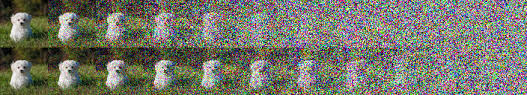
\includegraphics[width=\textwidth]{variance_schedule.jpeg}

As noted, the cosine schedule leads to a more gradual noising process.

\section{Network Model}

There are several different choices for the network architecture of \(P\), ranging from UNets \cite{ho_denoising_2020} to transformers \cite{tevet_human_2022}. Unfortunately, these models are unsuitable for most single-instance training due to their large receptive fields and global attention layers. Dealing with only a single training example can lead to overfitting to the training input, which can impact the diversity of generated results. However, recent work has shown that it is possible to replicate the performance of transformer-based networks using a more lightweight convolutional neural network architecture called CovNext \cite{liu_convnet_2022}. 

\subsection{Network architecture of P}
These CovNext modules form the backbone of the neural network \(P\), with residual connections to mitigate the vanishing gradient problem. The number of CovNext layers is a hyperparameter that can be adjusted depending on the use case. Increasing the depth of the network this way leads to more coherent motions at the cost of output diversity. The model uses a CovNext backbone depth of 16 after some empirical testing since it strikes a good balance between both goals.

The network also includes a time-step embedding layer, using a standard positional encoding scheme \cite{nikankin_sinfusion_2023}, that is added into the input of each CovNext module. This is key because the time-step in the diffusion process directly controls how much the input motion is noised, and thus the neural network needs access to this time-step information in order to denoise accordingly. Thus, the overall model for the denoising neural network \(P\) looks like the following:

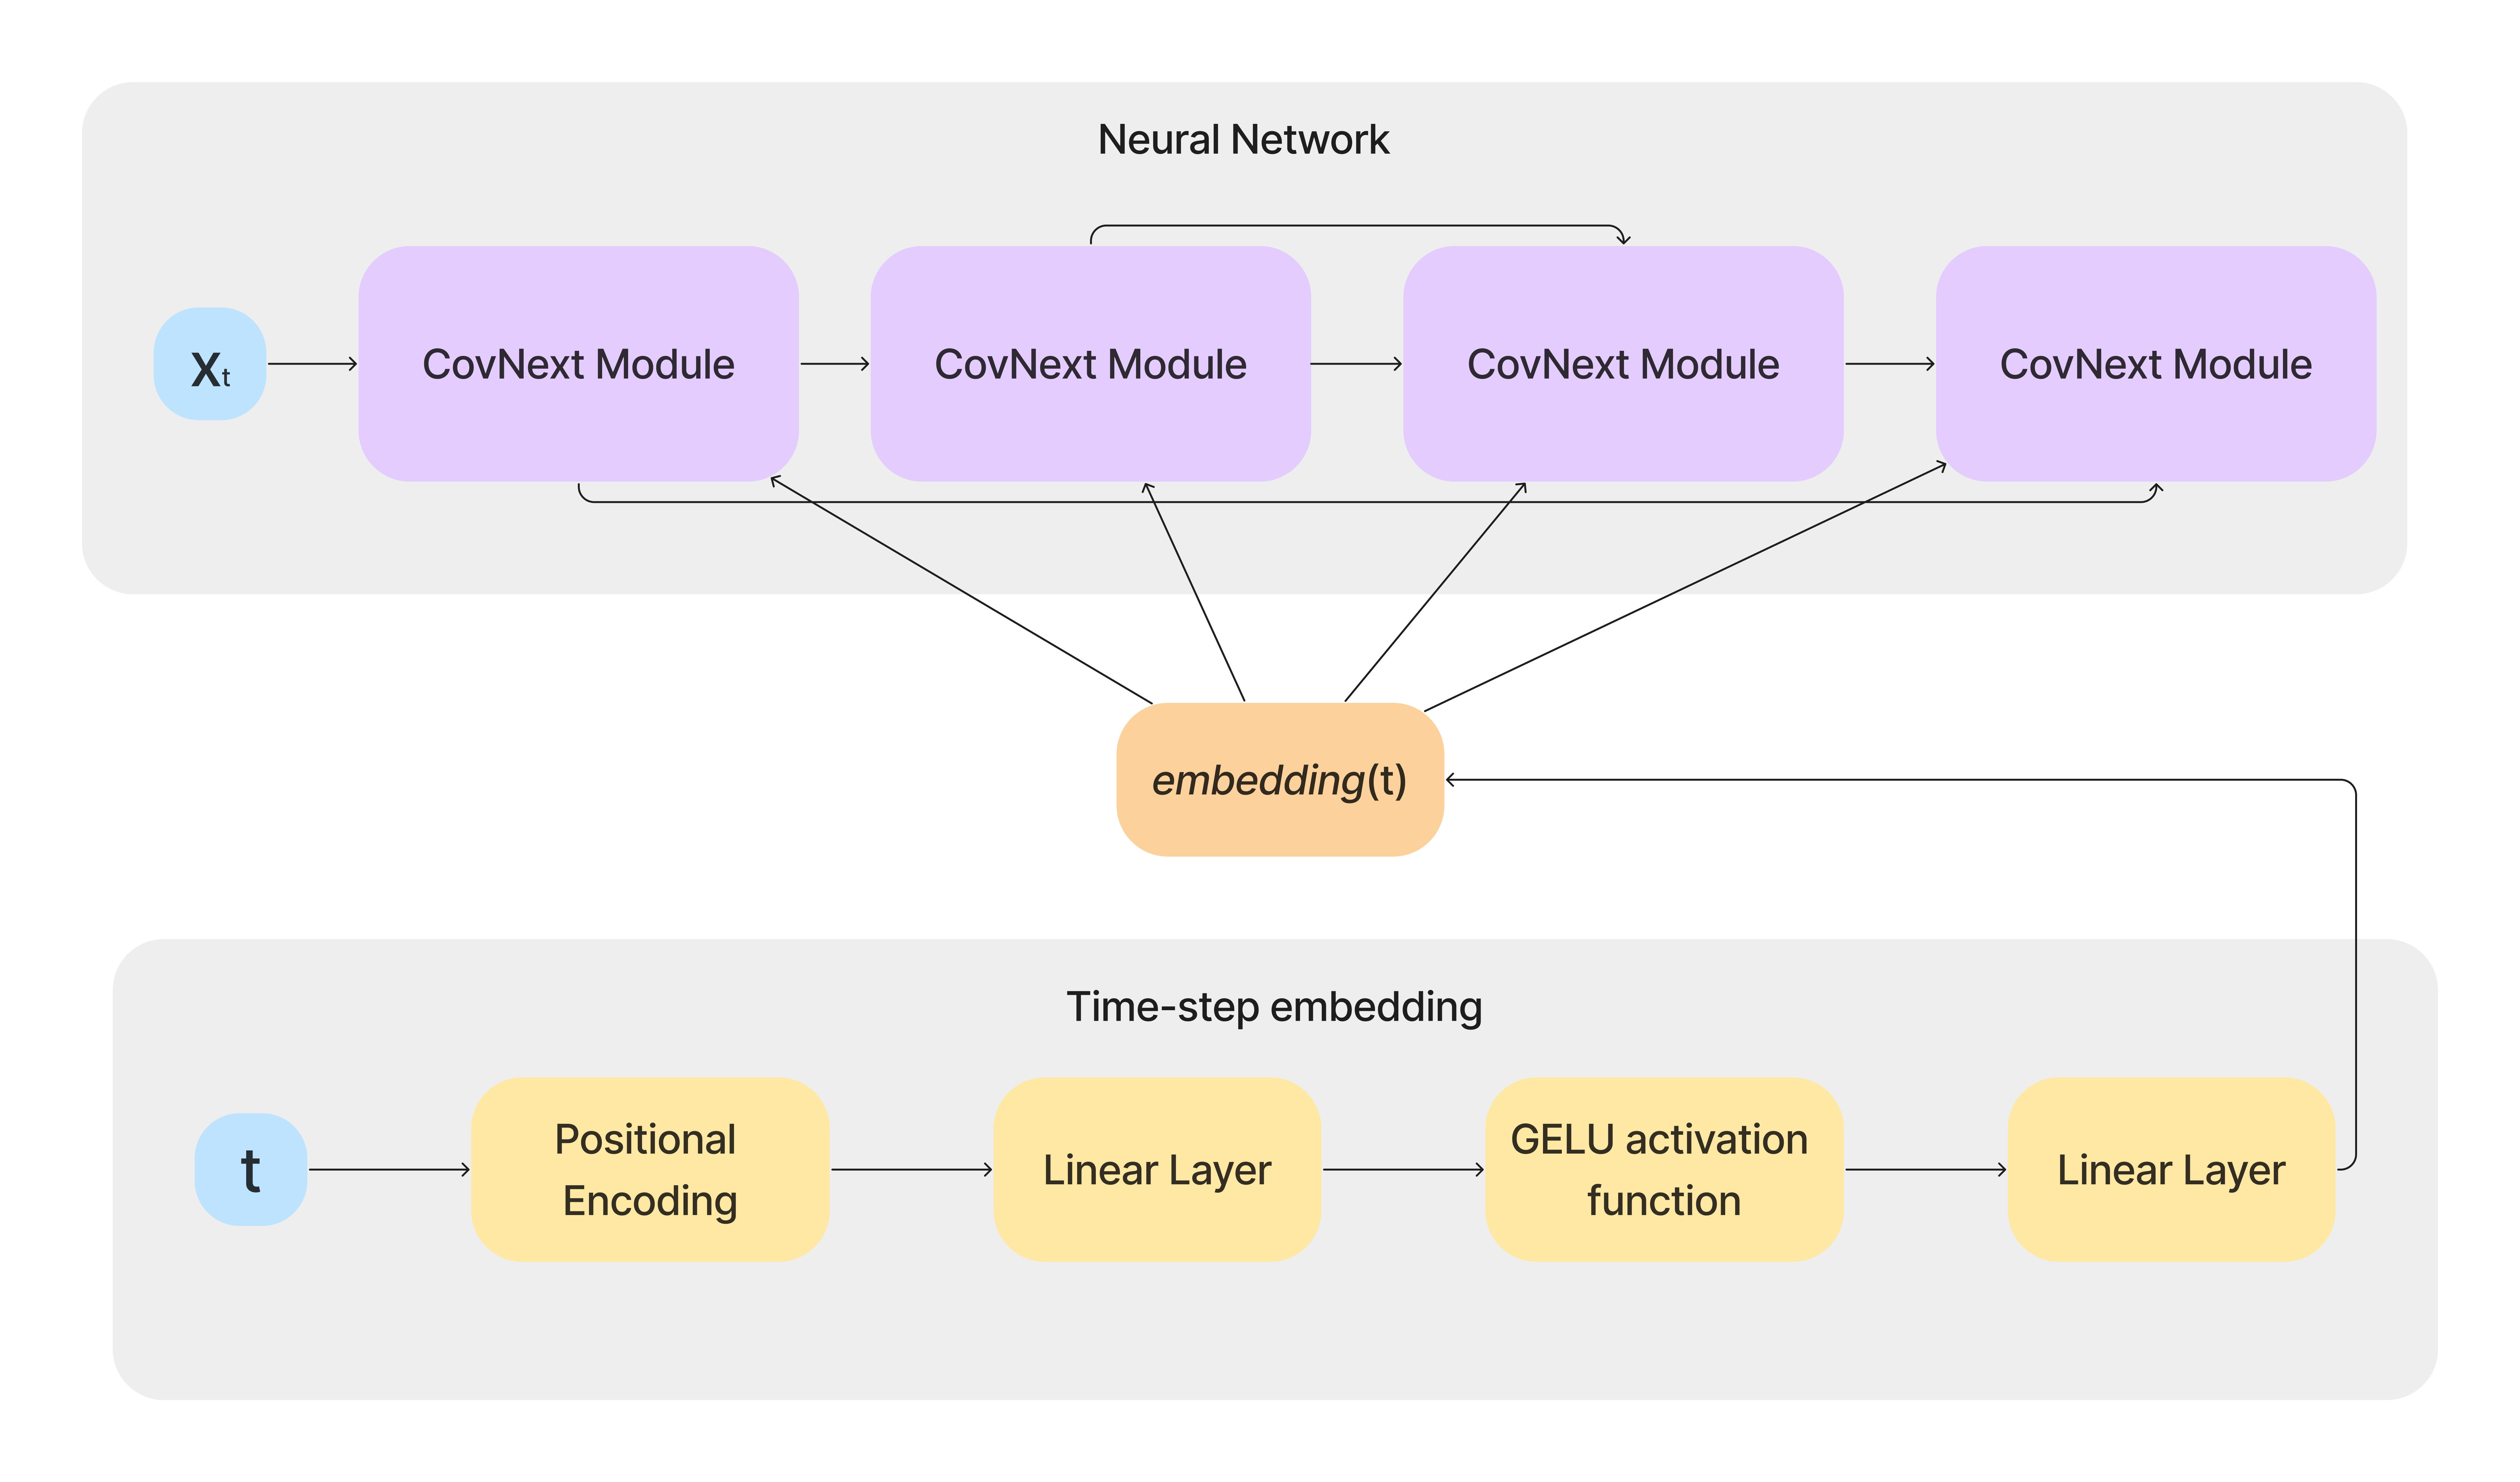
\includegraphics[width=\textwidth]{network_architecture.png}

\subsection{Dataset}

Since the model is trained on a single training example, the exact dataset used doesn't matter too much, and motions from different datasets could be feasibly combined. However, the model solely uses the Truebones Zoo BVH dataset \cite{truebones_free_2020} since all the motions within adhere to a fixed format, making the parser design simpler and less prone to error. The dataset contains motions of many different animals, allowing the model's performance to be tested on a variety of skeletons 

To parse, a simple top-down parser is used, and the properties of the BVH file are loaded into an intermediate class that specifies the joints, joint parents, frame information, rotation information for each frame and joint and more. All the relevant motion data is transformed into the input tensor according to \ref{motion-tensor}. Namely, a tensor is constructed by iterating over all joints in the order they were encountered and populating the rows with the appropriate rotation features using the 6D rotation representation. Then, the resulting 2D matrices are concatenated over all the frames in the motion, yielding a 3D tensor. The model also implements a coordinate change module to freely change between Euler angle, quaternion and 6D representations of rotations during the tensor construction step. This allows comparisons on how different rotation representations can affect model convergence and performance. 

\subsection{Training}
To train the model, a time-step \(t\) is uniformly sampled between 1 and \(T\). This is used to generate a noised version of the initial motion \(x_t\) according to \ref{sample-noised-directly}. This is implemented by a Diffusion class in the code that implements the diffusion algorithms to noise a given tensor \(x_0\) to a randomly generated time-step \(t\), yielding the noised version \(x_t\). The CovNext-based denoising network \(P\) receives \(x_t\) and \(t\), and gives a prediction of the initial motion \(\hat{x_0}\). Then, the \(L_2\) loss defined in equation \ref{loss-function} is used to take a gradient descent step on the weights of \(P\). We repeat this process, randomly sampling a new time-step each time until the weights of the neural network \(P\) converge:

\begin{algorithm}[H]
	\caption{Training neural network P} \label{training-pseudocode}
	\begin{algorithmic}[1]
		\Repeat
		\State \(t \sim \mathcal{U}(1, T)\)
		\State \(\epsilon \sim \mathcal{N}(0, I)\)
		\State \(x_t = \sqrt{\bar{\alpha_{t}}}{x_0} + \sqrt{1 - \bar{\alpha_{t}}} \epsilon\)
		\State \(\hat{x_0} = P(x_t, t)\)
		\State Gradient Descent on:
		\(\nabla{||x_0 - \hat{x_0}||}^2\)
		\Until weights of P converged
	\end{algorithmic}
\end{algorithm}

The model is implemented in the PyTorch library and trained on an Nvidia 3060 12GB graphics card. In the model, the number of diffusion steps \(T\) is set to 1000, using a cosine scheduler for the variance as previously explained. The model is trained on a batch size of 64, using the Adam optimizer with the default learning rate of \(0.001\). 

Since only a single training example is used, each element of the batch is the same initial input but undergoes an independent noising process, leading to more robust model convergence. Finally, to avoid the training process taking too long, the number of iterations of algorithm \ref{training-pseudocode} is capped at 50,000 iterations, which empirically leads to acceptably small losses at the end.

\chapter{Evaluation}

\section{Evaluation Metrics} \label{metrics}
The fields of single-instance training and motion generation are still relatively new and don't have standard evaluation metrics such as in the image generation domain. However, there are broadly two goals of the model, namely, generating motions that are coherent and generating motions that are diverse. 

These goals are somewhat contradictory since coherence involves evaluating how plausible the generated motion is given the input motion, while diversity involves making the outputs as different from the training input as possible. This trade-off between metrics is a common problem in many ML papers and is usually solved by calculating the harmonic mean of the all metrics. For example, the popular F1 score used in classification task is a specific type of harmonic mean \cite{hicks_evaluation_2022}. Generalizing this idea, the model is evaluated based on certain metrics and the harmonic mean score of these metrics is calculated as follows:

\begin{equation} \label{harmonic-mean}
	Harmonic Mean Score = \dfrac{M}{\sum_{n=1}^M \dfrac{1}{s_n}}
\end{equation},

where \(M\) is the total number of metrics and \(s_n\) is the score of the \(nth\) metric. 

The metrics used to evaluate the model are derived from similar works in the field \cite{li_ganimator_2022} and aim to quantitatively measure the two goals of the model:

\subsection{Coherence Score} \label{coherence}
To evaluate coherence of generated results, it is useful to measure how much of the input motion is reproduced by the generated motion. The more of the input is reproduced by the generated result, the more coherent it is as it more closely follows the intended data distribution. However, this is difficult to measure in the realm of animation, where the data not only varies spatially in terms of the joint positions but also varies temporally across frames, where the number of all possible windows across frames is extremely large. 

Using the convention from other papers dealing with motion generation, a fixed length \(s\) is chosen for the the length of the frame windows to make the problem more tractable \cite{li_ganimator_2022}. To evaluate, a length of \(s=24\) is chosen, which corresponds to 1 second of continuous animation in the Truebones Zoo dataset, since it has a frame time of 24 fps. Using this, all possible 24-frame windows in our inputs can be computed. For example, for a motion sequence \(M\) with a length of \(l\) frames, the set of all possible 24-frame windows \(\mathcal{W}(M)\) is:  
\begin{equation}
	\mathcal{W}(M) = \{ M_1:M_{24}, M_2:M_{25},\dots, M_{l-22}:M_{l-1}, M_{l-23}:M_l\},
\end{equation}

where \(M_i\) specifies the \(i\)th frame in the motion sequence \(M\), and \(M_i:M_j\) specifies the collection of frames between the \(i\)th and \(j\)th frame of \(M\) inclusive.

For the model, the set of all possible 24-frame windows of the initial motion sequence \(\mathcal{W}(x_0)\) and the generated output \(\mathcal{W}(\hat{x_0)}\) is calculated using a simple sliding window algorithm that iterates over the motion sequences linearly. Once these sets are constructed, it is determined what what percentage of all the windows in \(\mathcal{W}(x_0)\) are reproduced by the windows in \(\mathcal{W}(\hat{x_0)}\). 

To determine whether a window \(w \in \mathcal{W}(x_0)\) is reproduced, its nearest neighbour \(w_{nn} \in \mathcal{W}(\hat{x_0)}\) is found to calculate if the distance between them is less than a certain pre-determined threshold \(\epsilon\). For the model, the threshold is set to \(\epsilon=2\) based on empirical testing.

An important consideration is how the distance between two windows is calculated, which is required for determining the nearest-neighbour, via a simple linear scan, and calculating if the nearest-neighbour is within the threshold. The algorithm used to calculate distances between windows is simply based on the Euclidean distance between joint positions across all frames:

\begin{algorithm}[H]
	\caption{Calculating distance between windows \(a\) and \(b\)} \label{distance-metric}
	\begin{algorithmic}[1]
		\State \(F = \) number of frames in \(a\)
		\State \(J = \) number of joints in skeleton
		\State sum = 0
		\For{\(f = 1, \dots, F\)}
		\State \(a_f\) = \(f\)th frame of \(a\)
		\State \(b_f\) = \(f\)th frame of \(b\)
		\For{\(j = 1, \dots, J\)}
		\State \(a_{fj}\) = 3D coordinate of \(j\)th joint in \(a_f\)
		\State \(b_{fj}\) = 3D coordinate of \(j\)th joint in \(b_f\)
		\State sum += \({||a_{fj} - b_{fj}||}^2\)
		\EndFor
		\EndFor
		\State \Return (sum / (F * J))
	\end{algorithmic}
\end{algorithm}

Finally, the percentage of windows that are reproduced in the set \(\mathcal{W}(x_0)\) is calculated to give a coherence score, where a higher score corresponds to more coherent results.

\subsection{Diversity score}
To evaluate diversity, it is key to measure how different the generated motions are to the input training motion. As mentioned in chapter \ref{coherence}, this is difficult for data that operates on both a temporal and spatial level, and so the same strategy of slicing the motions into 24-frame windows is used. Once  the set of windows \(\mathcal{W}(x_0)\) and \(\mathcal{W}(\hat{x_0)}\) is determined, the following metric is defined for evaluating diversity. For each window in the generated motion \(\hat{w} \in \mathcal{W}(\hat{x_0})\), its nearest neighbour in the training motion \(w_{nn} \in \mathcal{W}(x_0)\) is determined using the distance metric defined in algorithm \ref{distance-metric} via a linear scan process. Then, the following formula is used to find the average distance between windows in the generated motion and its nearest neighbour in the training motion for all windows in the set:

\begin{equation} \label{diversity-score}
	\dfrac{\Sigma_{\hat{w} \in \mathcal{W}(\hat{x_0})} distance(\hat{w}, NearestNeighbour(\hat{w}))}{|\mathcal{W}(\hat{x_0})|}
\end{equation}

If the average distance is high, it means that the windows in the generated motions are quite different compared to windows in the training motion, which indicates a high diversity in the output. If the average distance is low, it means that the generated motion closely matches some windows in the training motion, which means it either overfits the training motion or it collapses to a static pose in the training motion. Thus, the result of equation \ref{diversity-score} is used as the diversity score, where a higher score corresponds to more diverse results.

\section{Evaluation Results}
To evaluate our results, both qualitative and quantitative findings are presented, with additional ablation studies to evaluate the model architecture choices.

\subsection{Qualitative Results}
For the qualitative evaluation, the model is trained on a motion of a spider attacking. The model is fully trained once and used to generate 5 motion samples of equal frame length as the training input. Then, the generated BVH file is imported into Blender \cite{blender_blenderorg_2024} to render a 3D model of the motion from a fixed perspective. The number of frames in the animations is too high to present properly, so the figures below are limited to the first 3 and last 3 frames of the entire motion sequence:
\begin{figure}[H]
	\centering
	
\includegraphics[width=\textwidth]{GeneratedMotions/image_reel_03.png}
	\caption{Training motion sequence}
	\label{training_image}
\end{figure}

\begin{figure}[H]
	\centering
	
\includegraphics[width=\textwidth]{GeneratedMotions/image_reel_00.png}
	\caption{Generated motion sequence 1}
	\label{image_00}
\end{figure}

\begin{figure}[H]
	\centering
	
\includegraphics[width=\textwidth]{GeneratedMotions/image_reel_01.png}
	\caption{Generated motion sequence 2}
	\label{image_01}
\end{figure}

\begin{figure}[H]
	\centering
	
\includegraphics[width=\textwidth]{GeneratedMotions/image_reel_02.png}
	\caption{Generated motion sequence 3}
	\label{image_02}
\end{figure}

\begin{figure}[H]
	\centering
	
\includegraphics[width=\textwidth]{GeneratedMotions/image_reel_initial.png}
	\caption{Generated motion sequence 4}
	\label{image_03}
\end{figure}

\begin{figure}[H]
	\centering
	
\includegraphics[width=\textwidth]{GeneratedMotions/image_reel_04.png}
	\caption{Generated motion sequence 5}
	\label{image_04}
\end{figure}

From the figures above, it can be seen that generated motions are all distinct from each other but still follow the same general motions as the initial training input. Furthermore, the transitions between poses are coherent and do not exhibit jittering or unnatural cuts, leading to a more plausible motion. 

Another interesting thing to note is that the first 3 frames of all the motions are quite similar to each other, while the last 3 frames differ quite significantly as the random changes to the rotations and positions accumulate over time. This behaviour is ideal for the model, since the results are initially quite coherent and similar to the input motion but naturally transition into diverse motions by the end of the sequence. 

Furthermore, unlike the majority of motion generation models, the model is able to work on arbitrary non-humanoid skeletons such as spiders. The wide applicability of the model can be seen in the next example, where it is instead trained on a motion of a centipede. The model is able to generate diverse motions for this skeleton as well, but the total number of frames for each generated motion is also varied. This is particularly useful for crowd animation, where motions with the same frequencies would seem unnaturally in sync. 

By varying the motion lengths, the motions look more random and natural, while still following the general theme of the motion they were trained on. Furthermore, for crowd animation, it is undesirable for the initial poses to match each other too closely and the depth of the CovNext-based denoising network is reduced by half to decrease the generated motion's coherence to the initial input:
\begin{figure}[H]
	\centering
	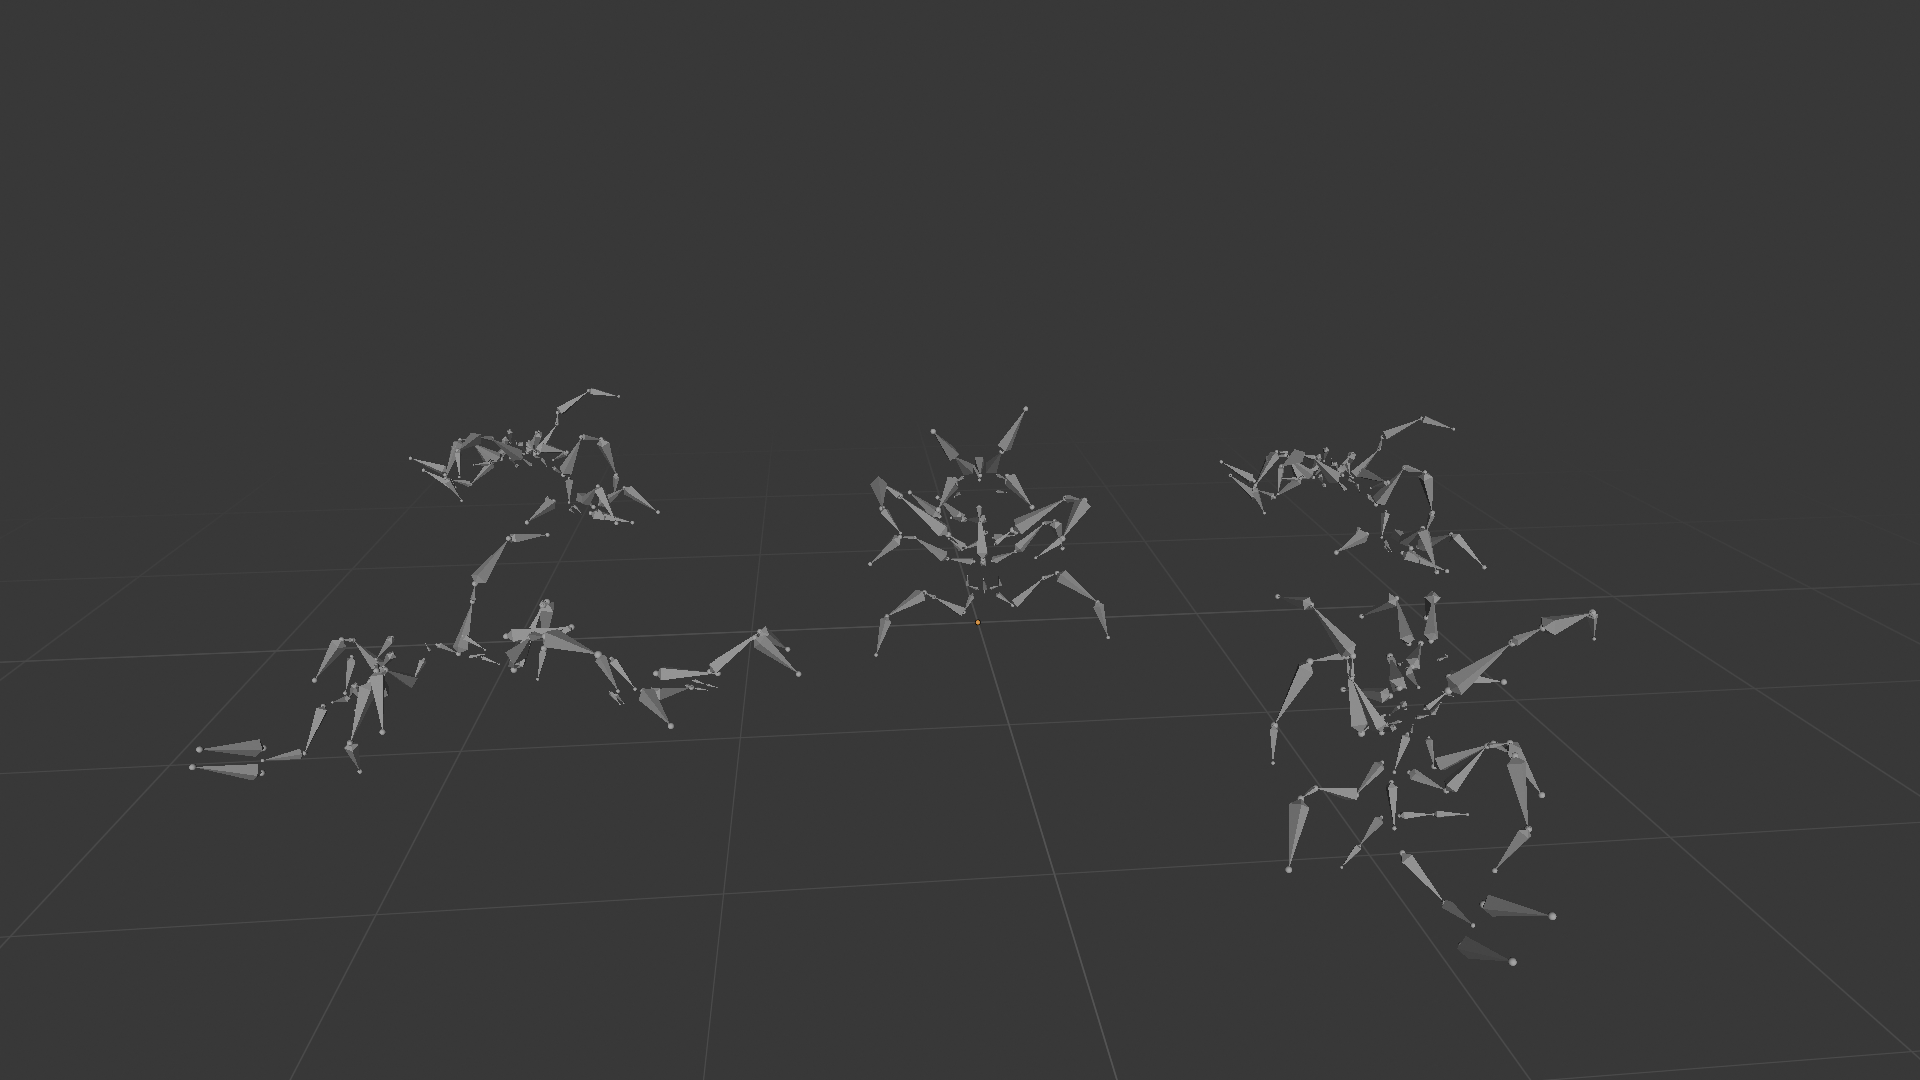
\includegraphics[width=\textwidth]{GeneratedMotions/CrowdAnimation0001.png}
	%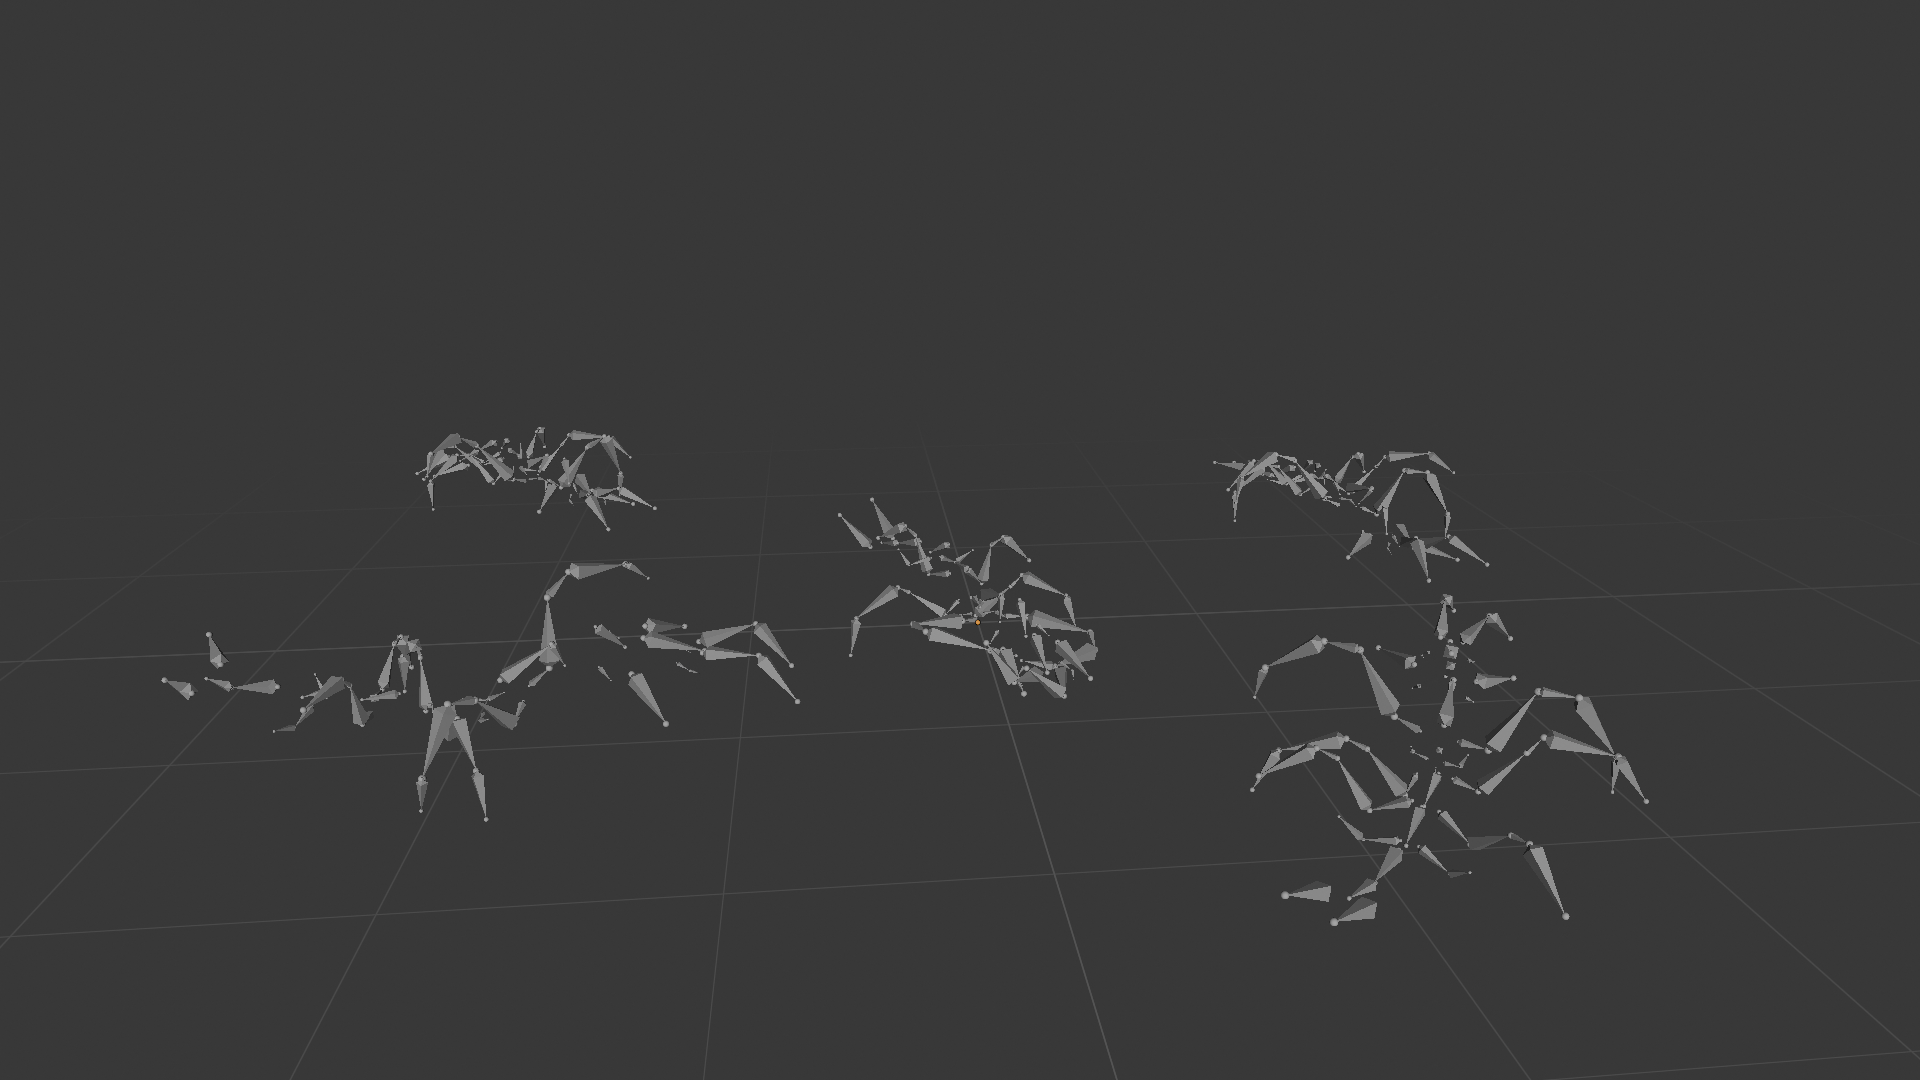
\includegraphics[width=\textwidth]{GeneratedMotions/CrowdAnimation0002.png}
	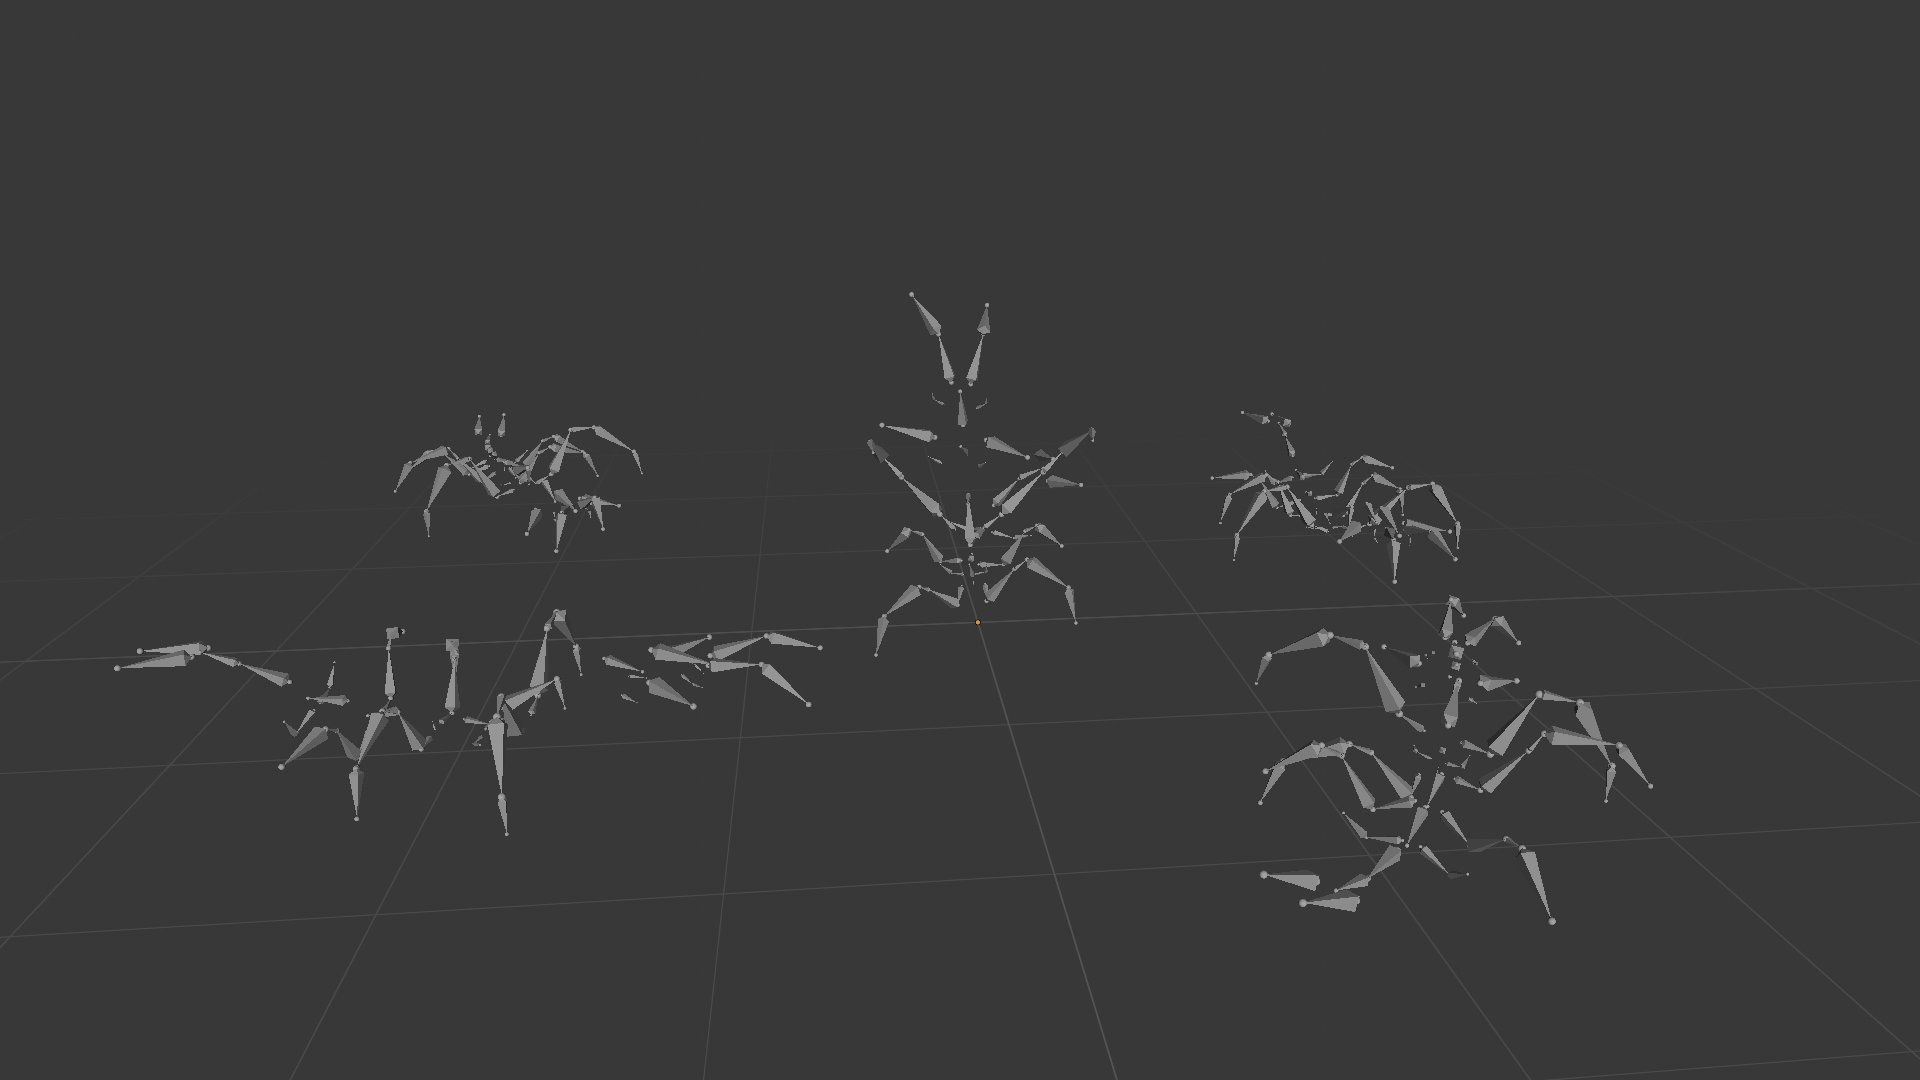
\includegraphics[width=\textwidth]{GeneratedMotions/CrowdAnimation0003.png}
	\caption{Crowd animation from single training example}
	\label{crowd_animation}
\end{figure}

The motions are all generated from the same training example, and imported into Blender with random root positions and rotations, yielding a convincing crowd animation. The first image displays the first frame of the animation, while the second image corresponds to the last frame of the animation. Note how all the poses are distinct from each other in the first and last frames, owing to the low denoising network depth. 

\subsection{Quantitative Results}
For the quantitative results, the metrics defined in section \ref{metrics} are used. To calculate a more representative score, the model is trained separately on 5 distinct training motions with different skeletons, using the model choices and hyperparameters discussed throughout chapter \ref{chap_implementation}.

For each training motion, 5 motions from the trained model are generated. Then, the arithmetic mean of the reproduction and diversity scores of the motions are calculated. Finally, the reproduction and diversity scores across all training motions are average to yield a representative result of how well the model scores on a range of different skeletons.

To balance the metrics of reproduction score and diversity score, the harmonic mean score defined in equation \ref{harmonic-mean} is used to calculate how well the model balances coherence and diversity. A high harmonic mean score indicates a good balance of both goals. The result on the model as defined is as follows:

\begin{table}[H]
	\centering
	\begin{tabular}{||c c c c||} 
		\hline
		Training Motion  & Reproduction Score & Diversity Score & Harmonic Mean Score \\ [0.5ex] 
		\hline\hline
		1                & 88.4               & 1.06            & 2.09                \\ 
		2                & 90.2               & 1.03            & 2.03                \\
		3                & 89.7               & 1.09            & 2.15                \\
		4                & 87.9               & 1.11            & 2.19                \\
		5                & 90.5               & 1.05            & 2.07                \\
		\textbf{Average} & \textbf{89.34}     & \textbf{1.07}   & \textbf{2.11}       \\[1ex] 
		\hline
	\end{tabular}
\end{table}

The high reproduction score indicate that the model is very coherent and learns the themes of the training motion well. However, it also has a positive diversity score and harmonic mean score, indicating that it does not overfit to the training motion or collapse to a static pose and balances the two goals of the model well. 

\subsection{Ablation study}
To justify the model choices made in chapter \ref{chap_implementation}, an ablation study is performed to measuring the metrics above after making certain changes to the model. Namely, these changes include changing the variance schedule to use a linear schedule, changing the rotation representations to quaternions and Euler angles, and changing the depth of the CovNext denoising network \(P\). The results of this ablation study are presented below:

\begin{table}[H]
	\centering
	\begin{tabular}{||c c c c||} 
		\hline
		Model type           & Reproduction Score & Diversity Score & Harmonic Mean Score \\ [0.5ex] 
		\hline\hline
		Default              & 89.34              & 1.07            & 2.11                \\ 
		Linear schedule      & 85.09              & 1.00            & 1.98                \\
		Quaternions          & 87.63              & 1.04            & 2.06                \\
		Euler angles         & 86.28              & 1.04            & 2.06                \\
		Double CovNext depth & 94.06              & 1.01            & 2.00                
		\\[1ex] 
		\hline
	\end{tabular}
\end{table}

From the table above, it is clear that the default model choices strike the best balance between coherence and diversity, yielding the highest harmonic mean score. An interesting thing to note is that the rotation representations do not make as much of a difference as expected, yielding similar scores across metrics to the default 6D rotation representations. This might be because of the small sample size, and perhaps the change would be more obvious across more types of skeletons and longer motion sequences that give time for rotation errors to accumulate. 

The biggest impact to model performance comes by changing the variance schedule from cosine to linear. This makes sense since the linear schedule is proven too be a lot more destructive in the noising process, causing the denoising model to struggle \cite{nichol_improved_2021}. Interestingly, the linear schedule model scores low in both the reproduction score and diversity score, indicating that it collapses to a pose that it not even representative of the training motion. Lastly, the change to CovNext depth is as predicted by several papers, where increased depth leads to a higher receptive field, leading to overfitting to the input at the expense of diversity. 

\chapter{Conclusions}
\section{Achievements}
The project successfully implements a model to generate new motions given only a single training input. This allows the generation of motions of arbitrary skeletons, which is useful in fields such as animation and video games, and can significantly reduce the need for manual animation rigging. The model uses the noising and denoising diffusion processes from the state-of-the-art diffusion model that has seen tremendous success in the image domain. It uses this process to train a neural network \(P\) that can denoise from pure noise to generate plausible motions that match the input training motions. 

The architecture of the neural network is carefully considered to mitigate issues with single-instance training such as large receptive fields and overfitting. This is done by utilizing a CovNext-based backbone for the network, a strategy that has seen success for other single-instance training tasks. The network also includes time-step embedding layers to be able to conditionally train on noising time-step, and thus learn how to denoise from arbitrary time-steps in the diffusion process.

The results of the model are then evaluated qualitatively and quantitatively, alongside an ablation study to justify model hyperparamaters and architecture choices. However, the task of evaluating motion data is a difficult one due to how it varies both spatially and temporally. Thus, works from similar motion generation papers are used to define bespoke metrics to evaluate model performance, namely, the reproduction score and the diversity score. These scores successfully quantify how well the model achieves its goals of generating diverse and coherent motions, and they give a deeper insight into how changes to the model affect its results.

\section{Future Work}
The promising results achieved by the current model suggest several avenues for further research and development. A potential enhancement is the creation of a conditional version of the model. Specifically, conditioning the model on external inputs, such as joystick movements or other user interactions, could significantly enhance its applicability in interactive scenarios like video games or virtual reality, where user input directly influences motion generation in real-time.

Integrating a foot contact loss function \cite{tevet_human_2022} could also be highly beneficial, especially for datasets that lack explicit contact information. This integration would improve the physical plausibility of the generated motions by ensuring that foot placements are realistic and appropriately grounded, thus reducing floating or sliding artifacts that often detract from visual realism.

Moreover, advancing the evaluation methods used to assess the quality of generated motions by incorporating physics-based metrics is proposed. Utilizing forward kinematics could provide a more accurate measurement of the deviation of generated motion from expected physical behavior. 

\appendix

\printbibliography

\chapter{Project Plan}

\includepdf[pages=-,scale=.8,pagecommand={}, frame]{Project Plan.pdf}

\chapter{Interim Report}
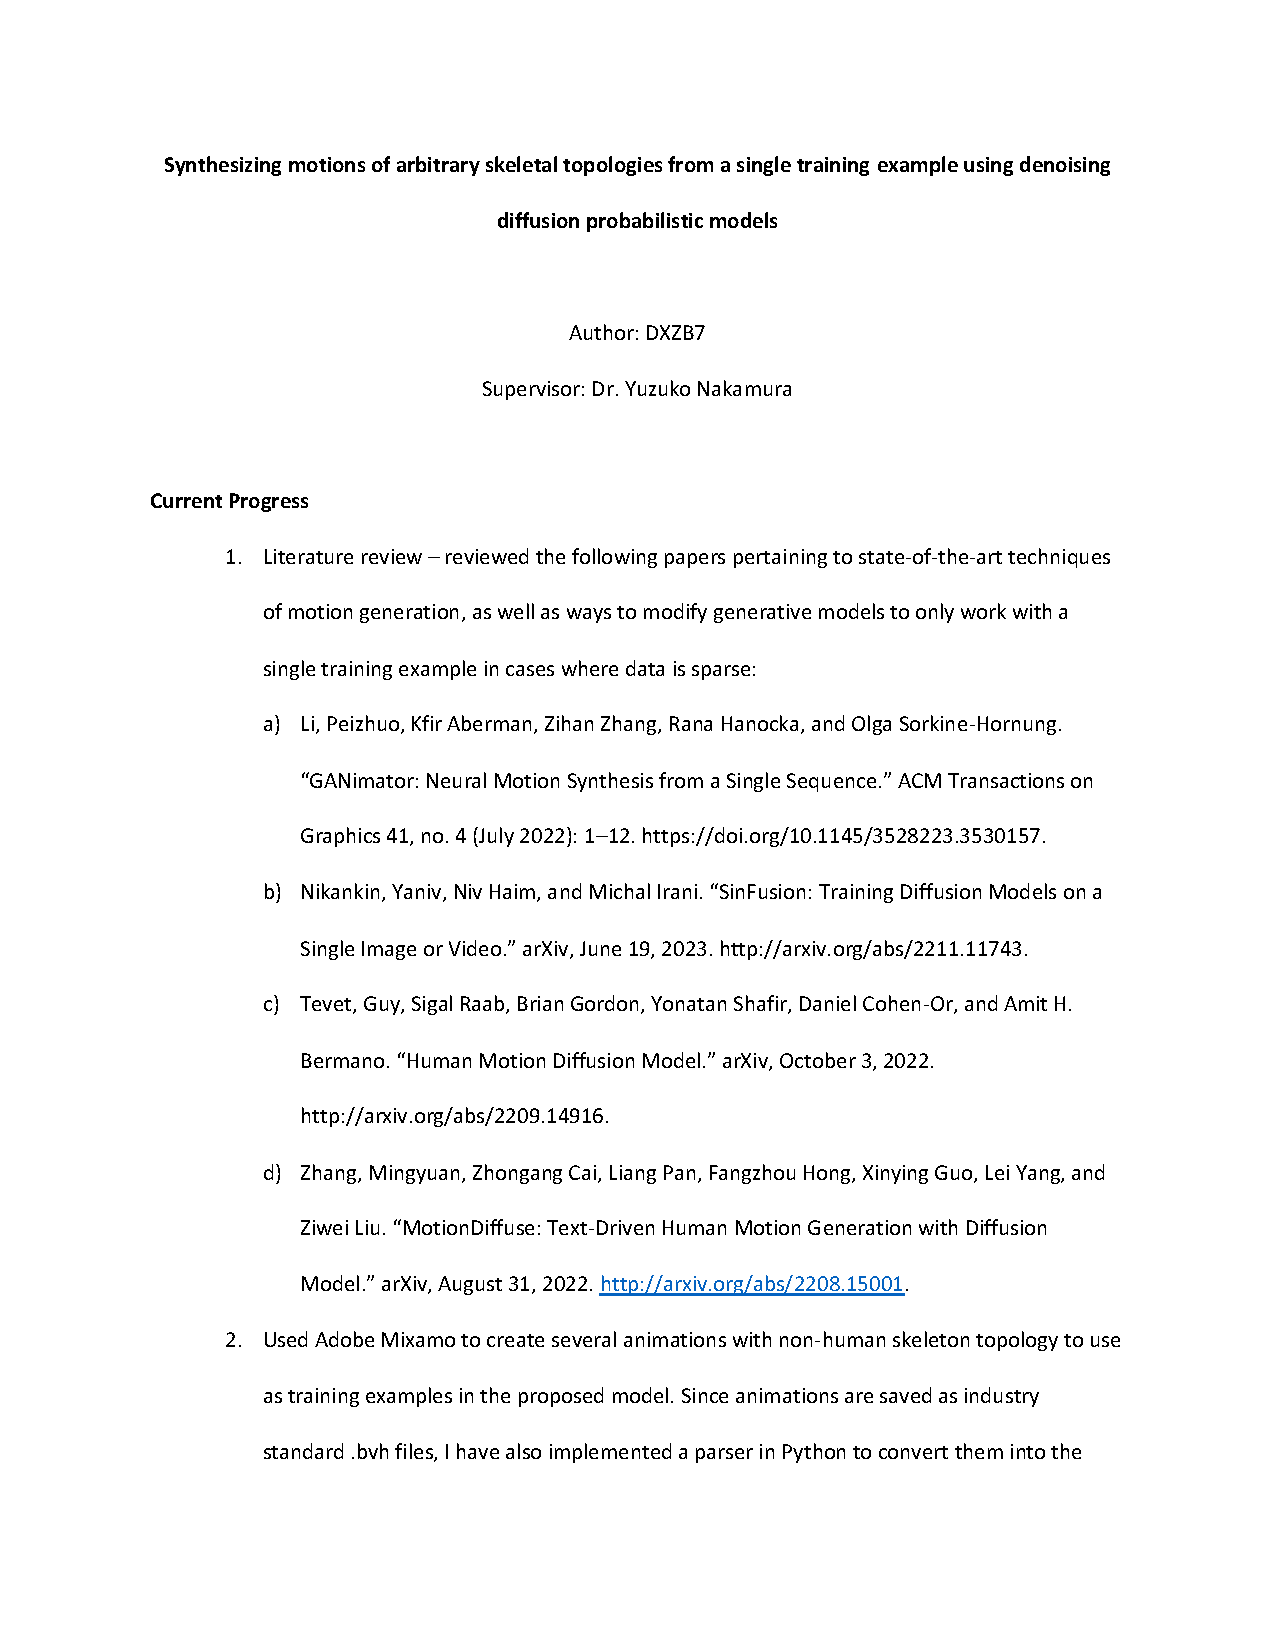
\includepdf[pages=-,scale=.8,pagecommand={}, frame]{UCl Final Year Project Interim Report.pdf}

\chapter{Source code}

\lstinputlisting[language=Python, caption=train.py]{Code/training/train.py}
\lstinputlisting[language=Python, caption=transforms.py]{Code/transforms/transforms.py}
\lstinputlisting[language=Python, caption=diffusion.py]{Code/models/diffusion.py}
\lstinputlisting[language=Python, caption=nextnet.py]{Code/models/nextnet.py}
\lstinputlisting[language=Python, caption=getmotiondata.py]{Code/dataloader/getmotiondata.py}
\lstinputlisting[language=Python, caption=load.py]{Code/bvh/load.py}

\end{document}